\documentclass[FisicaTeorica.tex]{subfiles}
\begin{document}
\chapter{Descrizione matematica di un sistema fisico}
\vspace{-1em}
(\textbf{DISCLAIMER}: Questo appunto contiene ricerca personale, e quindi potrebbero esserci scritte cavolate. Attenzione!) \\ \lesson{3}{04/10/2018}
Ci occupiamo ora di introdurre il \textbf{formalismo matematico} che utilizzeremo per descrivere i \textbf{sistemi fisici} in Meccanica Quantistica. In particolar modo, ci servirà definire gli \textbf{enti fisici} (osservabili e stati) che caratterizzano il sistema, e le \textbf{regole} a cui obbediscono (valor medio ed evoluzione temporale). Ci concentreremo sul perché la \MQ  renda necessario ridefinire cose apparentemente \textit{ovvie}, lasciando in sospeso alcune importanti questioni che saranno opportunamente riprese e concluse nel prossimo capitolo.\\
\section{Osservabili}
Si definiscono \textbf{osservabili}\footnote{\textit{Sostantivo femminile}} \marginpar{Osservabile} le quantità fisiche $O$ che possiamo misurare in linea di principio (ad un certo istante), come ad esempio \textit{posizione}, \textit{impulso}, \textit{energia}.\\
Lo \textbf{spettro} $\sigma(O)$ dell'osservabile $O$ è l'insieme dei valori che possiamo ottenere con una misura di $O$. Ovviamente deve essere $\sigma(O) \subseteq \bb{R}$, in quanto lo spettro di un osservabile deve essere confrontabile con l'esperimento, e le misure sono numeri reali.\\

\begin{center}
\tikzset{every picture/.style={line width=0.75pt}} %set default line width to 0.75pt        
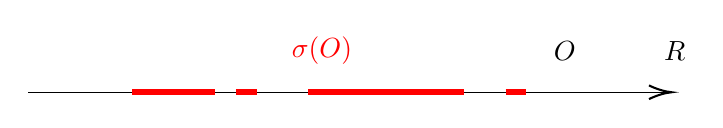
\begin{tikzpicture}[x=0.75pt,y=0.75pt,yscale=-1,xscale=1]
%uncomment if require: \path (0,300); %set diagram left start at 0, and has height of 300
%Straight Lines [id:da27846539722124186] 
\draw    (120,150) -- (428,150) ;
\draw [shift={(430,150)}, rotate = 180] [color={rgb, 255:red, 0; green, 0; blue, 0 }  ][line width=0.75]    (10.93,-3.29) .. controls (6.95,-1.4) and (3.31,-0.3) .. (0,0) .. controls (3.31,0.3) and (6.95,1.4) .. (10.93,3.29)   ;
%Straight Lines [id:da17770457076107338] 
\draw [color={rgb, 255:red, 255; green, 0; blue, 0 }  ,draw opacity=1 ][line width=2.25]    (170,150) -- (210,150) ;
%Straight Lines [id:da09934995394761348] 
\draw [color={rgb, 255:red, 255; green, 0; blue, 0 }  ,draw opacity=1 ][line width=2.25]    (220,150) -- (230,150) ;
%Straight Lines [id:da7555893739350281] 
\draw [color={rgb, 255:red, 255; green, 0; blue, 0 }  ,draw opacity=1 ][line width=2.25]    (255,150) -- (330,150) ;
%Straight Lines [id:da6066958001552576] 
\draw [color={rgb, 255:red, 255; green, 0; blue, 0 }  ,draw opacity=1 ][line width=2.25]    (350,150) -- (360,150) ;
% Text Node
\draw (378.5,130) node   {$O$};
% Text Node
\draw (261.5,130) node [color={rgb, 255:red, 255; green, 0; blue, 0 }  ,opacity=1 ]  {$\sigma ( O)$};
% Text Node
\draw (431.5,130) node   {$\mathbb{R}$};
\end{tikzpicture}
\end{center}

In \textbf{Meccanica Classica} (\MC), nel formalismo hamiltoniano, ad un sistema sono associate le coordinate $q=\langle q_1,\dots, q_n\rangle$ (posizioni) e i momenti coniugati $p=\langle p_1,\dots, p_n\rangle$, dove $n$ è il numero di gradi di libertà. Lo spazio delle coppie $(q,p)$ è detto \textbf{spazio delle fasi} e lo denoteremo con $\Omega$.\\
Le osservabili sono \textit{funzioni reali} su $\Omega$ e formano un'algebra abeliana su $\bb{R}$, per addizione e moltiplicazioni puntuali (ossia, se ho un'osservabile $f(q,p)$ e una $g(q,p)$ esiste sempre l'osservabile-prodotto $(fg)(q,p)=f(q,p)g(q,p)$ e, essendo un'algebra abeliana, vale la proprietà commutativa $f(q,p)g(q,p)=g(q,p)f(q,p)$).\\
Tale struttura algebrica appena definita è necessaria perché osservabili che contengono prodotti per scalari, somme e prodotti di altre osservabili siano ben definiti. Un esempio è l'energia: $O=\mathcal{H}(q,p)=\frac{1}{2m} p\cdot p+V(q)$.\\
In \MC, inoltre, lo spettro $\sigma(f(q,p))$ è semplicemente il codominio della funzione $f$, ossia i valori che $f$ può assumere. Questa proprietà, intuitiva e tipica della \MC, non segue però dalla definizione di osservabile che abbiamo dato (non è detto che l'insieme dei valori ottenuti dalla misura siano gli stessi che può assumere l'osservabile).\\
\begin{comment}
\footnote{Nello specifico, questa è un'affermazione a posteriori, quando si scopre che in \MQ gli osservabili sono descritti da \textit{operatori}, per cui chiaramente l'insieme delle misure $\sigma(O)$ non può essere il \q{codominio} di un operatore - non ha senso! Infatti in questo caso vedremo che i valori dell'osservabile sono dati dalle soluzioni di equazioni agli autovalori in cui compare tale operatore. Un'osservabile, in matematica, è proprio l'\textit{entità fisica} che si misura, e deve riprodurne le caratteristiche. Non è per nulla scontato che un'osservabile \textit{rispecchi} le regole algebriche dei reali (es. come la somma di due reali è un reale, così la somma di due osservabili è un'osservabile): per la fisica classica ci va bene che sia così, e quindi ci pare intuitivo, ma scavando nel funzionamento dell'universo e arrivando alla \MQ ci si accorge che non è più così: anzi, continuare con le idee classiche produce contraddizioni con gli esperimenti!}).\\
\end{comment}
Riepilogando, in \MC:
\begin{enumerate}
    \item Le osservabili sono funzioni \textbf{reali}
    \item Lo spettro di un'osservabile è il \textbf{codominio} della funzione ad esso associata
    \item Le osservabili si possono sommare tra loro, dando luogo ad altre osservabili, e anche moltiplicare con \textbf{commutatività}
\end{enumerate}
Tutte queste proprietà, che sembrano estremamente ovvie, non necessiterebbero nemmeno di essere enunciate se non fosse che in Meccanica Quantistica (\MQ) vengono sistematicamente violate, come è stato verificato sperimentalmente.

\subsection{L'interpretazione di Heisenberg}
La prima intuizione in tal senso fu di Heisenberg (1925), partendo dalle regole della \textbf{spettroscopia} dell'atomo di idrogeno, per cui la frequenza delle righe di emissione è data dal principio combinatorio di Ritz-Rydberg:
\[
{\displaystyle {\frac {1}{\lambda }}=R\left({\frac {1}{n^{2}}}-{\frac {1}{m^{2}}}\right)}; \quad n,m \in \bb{N}
\]
Ogni frequenza $\omega$ può essere quindi indicizzata da due numeri $m,n$ come $\omega_{mn}$.\\
Ci si accorse di questa possibilità osservando che non tutte le frequenze facevano parte dello spettro dell'idrogeno (come ci si aspetterebbe in fisica classica), e quelle permesse avevano la proprietà di poter essere scritte sempre come differenza di numeri che non erano frequenze: $\omega_{mk} = \omega_m - \omega_k$.\\
Questo fatto è il prodotto della quantizzazione dell'energia degli elettroni: quando questi effettuano transizioni tra stati alti e stati bassi con energie fissate emettono un fotone di una determinata frequenza.\\
In particolare, notiamo che la somma di due frequenze (osservabili) non sempre corrisponde ad un'altra frequenza dello spettro. Più precisamente, la somma di due frequenze $\omega_{mk}$ e $\omega_{rs}$ porta ad una nuova frequenza permessa solo se $k=r$ o $m=s$, poiché in tal caso si effettua una \q{cancellazione}, visto che è possibile scomporre le frequenze come:
\[
\omega_{mk} + \omega_{rs} = \omega_m - \omega_k + \omega_r -\omega_s
\]
e sappiamo che le frequenze \q{accettate} sono differenze del tipo $\omega_i - \omega_j$. Se $k = r$, per esempio, avremo che $\omega_{mk} + \omega_{ks} = \omega_m - \omega_s = \omega_{ms}$.\\
Un qualsiasi formalismo adottato per la \MQ deve poter giustificare in maniera naturale tale fenomeno.\\
Heisenberg partì considerando una grandezza osservabile $q(t)$ periodica con frequenza fondamentale $\omega = 2\pi\nu$ (che potrebbe per esempio essere la posizione di un oscillatore armonico\footnote{Nel caso di una carica oscillante, potrebbe essere il \q{meccanismo} alla base dell'emissione delle righe dello spettro dell'idrogeno}), e la sua rappresentazione in serie di Fourier\footnote{Riferimento: \href{http://www.mathpages.com/home/kmath698/kmath698.htm}{http://www.mathpages.com/home/kmath698/kmath698.htm}}:
\[
q(t) = \dots + q_{-2}e^{-i2\omega t} + q_{-1}e^{-i\omega t} + q_0 + q_1 e^{i\omega t} + q_2 e^{i2\omega t} + \dots
\]
Per prima cosa dobbiamo assicurarci che, essendo $q(t)$ un'osservabile, sia reale. Per permettere questo una condizione sufficiente è $q_n = q_{-n}^*$ $\forall n\in \bb{Z}\setminus\{0\}$, cioè che se un coefficiente di Fourier $q_n = u_n + iv_n$, il suo \q{corrispondente} sia il suo complesso coniugato: $q_{-n} = q_{n}^* = u_n - iv_n$. Così facendo i termini immaginari di ogni coppia si cancellano:
\begin{align*}
q_n e^{in\omega t} + q_{-n}e^{-in\omega t} &= (u_n + iv_n)e^{in\omega t} + (u_n - iv_n)e^{-in\omega t} =\\
&= (u_n + iv_n)(\cos(n\omega t)+i\sin(n\omega t)) + (u_n-iv_n)(\cos(n\omega t) \bm{-} i\sin(n\omega t)) =\\
&= 2u_n\cos(n\omega t)-2v_n\sin(n\omega t)
\end{align*}
e il risultato $q(t)$ sarà reale.\\
È facile verificare che, se $a(t)$ e $b(t)$ rispettano questa proprietà, allora anche le loro somme la rispettano, e anche le loro derivate (come ci aspettiamo: la somma di reali è reale, la derivata di reali è reale).\\
Esaminiamone il prodotto, raccogliendo i termini con \q{la stessa periodicità}:
\begin{align*}
c(t) = a(t)b(t) &= \dots + (\dots +a_{-2}b_1 + a_{-1}b_0 + a_0 b_{-1} + a_1 b_{-2} + \dots )e^{-i\omega t} +\\
&+ (\dots +a_{-2}b_2 + a_{-1}b_1 + a_0 b_0 + a_1 b_{-1} + \dots ) + \\
&+ (\dots +a_{-1}b_2 + a_{0}b_1 + a_1 b_{0} + a_2 b_{-1} + \dots ) e^{i\omega t} + \dots
\end{align*}
(i termini con lo stesso esponenziale $ki\omega$ hanno come coefficiente la somma di prodotti del tipo $a_m b_n$ con $m+n=k$, poiché nella moltiplicazione gli esponenti vengono sommati).\\
Notiamo che anche il prodotto è reale: $c_{-k} = c_k^*$ in quanto l'uno è la somma dei coniugati dei termini dell'altro (ogni termine del tipo $a_m b_n$ nel coefficiente di $k$ avrà un analogo $a_{-m}b_{-n}$ nel coefficiente di $-k$, e il complesso coniugato di un prodotto è il prodotto dei complessi coniugati).\\
L'intuizione di Heisenberg fu nel rappresentare un'osservabile con una matrice le cui righe sono ripetizioni \q{shiftate} dei coefficienti della serie di Fourier, in modo che i coefficienti di ordine $0$ riempissero la diagonale principale:
\[
q(t) = \begin{pmatrix}
\ddots & \vdots & \vdots & \vdots & \vdots & \vdots & \iddots\\
\cdots & q_0 & q_1 e^{i\omega t} & q_2 e^{2i\omega t} & q_3 e^{3i\omega t} & q_4 e^{4i\omega t}  & \cdots\\
\cdots & q_{-1}e^{-i\omega t} &  q_0 & q_1 e^{i\omega t} & q_2 e^{2i\omega t} & q_3 e^{3i\omega t}  & \cdots\\
\cdots & q_{-2}e^{-2i\omega t} & q_{-1}e^{-i\omega t} &  q_0 & q_1 e^{i\omega t} & q_2 e^{2i\omega t} & \cdots\\
\cdots & q_{-3}e^{-3i\omega t} & q_{-2}e^{-2i\omega t} & q_{-1}e^{-i\omega t} &  q_0 & q_1 e^{i\omega t}  & \cdots\\
\cdots & q_{-4}e^{-4i\omega t} & q_{-3}e^{-3i\omega t} & q_{-2}e^{-2i\omega t} & q_{-1}e^{-i\omega t} &  q_0 & \cdots\\
\iddots & \vdots & \vdots & \vdots & \vdots & \vdots & \ddots\\
\end{pmatrix}
\]
Tale rappresentazione molto strana ha un suo perché, che ora esamineremo.\\
Sia $q_{mn}$ l'elemento di riga $m$-esima e colonna $n$-esima (qui valgono anche indici negativi). Per esempio $q_{00} = q_0$, e $q_{10} = q_1 e^{i\omega t}$. In generale:
\[
a_{mn} = a_{n-m}e^{i(n-m)\omega t}; \quad b_{mn} = b_{n-m}e^{i(n-m)\omega t}
\]
Vale poi $a_{mn} = a^*_{nm}$ (perché siamo partiti da una serie a somma reale).\\
È definita poi la somma di osservabili (sommando le matrici). Per il prodotto, invece, notiamo che, per $c(t) = a(t) b(t)$, il termine $c_{mn}$ è dato dal prodotto scalare tra la riga $m$-esima della matrice di $a$ e la colonna $n$-esima della matrice di $b$ (che sono uguali se non per il fatto che la seconda è \q{shiftata} di $n-m$ in avanti rispetto alla prima):
\[
c_{mn} = \sum_{\mu=-\infty}^\infty a_{m\mu} b_{\mu n}
\]
Esplicitiamo uno dei termini della somma:
\[
a_{m\mu}b_{\mu n} = a_{m-\mu}b_{\mu-n}e^{i(m-\mu) \omega t} e^{i(\mu-n)\omega t} = a_{m-\mu} b_{\mu-n}e^{i(m-n)\omega t} %Notazione doppio pedice e singolo pedice crea confusione!
\]
Perciò $c_{mn}$ avrà la stessa frequenza $(m-n)\omega$ di $a_{mn}$ e $b_{mn}$. Ma allora, concentrandoci solo sulle frequenze, dal calcolo di sopra notiamo che:
\[
\omega_{m\mu} + \omega_{\mu n} = \omega_{m n}
\]
Ora, nel caso che abbiamo costruito artificialmente (matrice della serie di Fourier), ciò è ovvio (deriva dal fatto che $\omega_{mn} = (m-n)\omega_0$, per costruzione). Tuttavia, Heisenberg considerò il caso più generale in cui tale espressione è verificata, che è quello in cui esistono determinate costanti $\omega_n$ tali che:
\[
\omega(m,n) = \omega_{m} - \omega_n
\]
%[TO DO] Integrare con appunti dell'altro canale (CFR teorema di Arnold)
Possiamo quindi modificare la matrice di prima cambiandone le frequenze seguendo questa regola appena trovata. Si otterranno colonne che non sono più serie di Fourier, ma un qualcosa di più generale - capace di spiegare gli spettri atomici trovati\footnote{Bisognerebbe anche eliminare tutti i termini con almeno un indice negativo, poiché si considerano transizioni solo tra \q{stati energetici positivi}.}.\\
Heisenberg congetturò che tutte le osservabili nell'atomo dovessero assumere la forma di termini di matrici, della forma $q_{mn}(t) = q_{mn}e^{i\omega_{mn}t}$ (dove $q_{mn}$ potrebbe essere, per esempio, l'intensità di una riga di emissione e $\omega_{mn}$ la sua pulsazione).\\
Ciò ha profonde conseguenze, poiché viola tutte le considerazioni intuitive fatte in \MC:
\begin{itemize}
    \item Le osservabili sono descritte da \textbf{matrici} con termini \textbf{complessi};
    \item Il prodotto tra osservabili è un prodotto matriciale (che non è detto neppure essere commutativo, dunque l'algebra non è abeliana).
\end{itemize}
%[Domanda]: Ma con osservabile si intende l'intera matrice o il singolo elemento dato dai due indici? E tali singoli elementi sono funzioni complesse? - Risposta (Marchetti): i due indici indicano l'elemento mn-esimo della matrice, e l'operatore va considerato come la matrice intera. In notazione, a volte si indica q(m,n) per l'intera matrice, immaginando di "far scorrere" gli indici con -\infty < n,m < +\infty
In effetti, confrontando questa intuizione con la quantizzazione di Planck, Heisenberg dimostrò che per un sistema unidimensionale, la posizione $q$, e il momento $p$ verificano:
\[
[q,p]_{mn} \equiv [qp - pq]_{mn} = i\hbar \delta_{mn}
\]
E cioè la commutatività viene meno (l'espressione tra parentesi è detta \textit{commutatore}).\\
Inoltre le matrici devono essere infinito-dimensionali. Infatti, se per assurdo le matrici fossero finito-dimensionali allora sarebbe definita una traccia, e dovrebbe valere:
\[
\op{Tr}(qp) = \op{Tr}(pq) \quad \Rightarrow \quad \op{Tr}(qp-pq) = 0 \neq \op{Tr}(i\hbar \bb{I}) = i \hbar
\]
($\op{Tr}$ è la traccia di una matrice), ovvero un assurdo.\\
L'unico modo perché le relazioni di commutazione siano consistenti è allora che la traccia non sia definita, e cioè che le matrici in questione siano infinito-dimensionali.\\

\subsection{L'approccio di Schrödinger}
Alle stesse conclusioni arrivò Schrödinger (1926) in modo più indiretto.\\
Scrivendo la sua equazione d'onda stazionaria per una particella con potenziale $V$:
\begin{equation}
    \left(\frac{{-\hbar}^2}{2m}\nabla^2\psi+V\psi\right)=\mathcal{E}\psi
    \label{eqn:onda}
\end{equation}
si accorse che si poteva ricondurre il membro di sinistra all'Hamiltoniana classica: 
\[H_\mathrm{cl}\left(\vec{x},\vec{p}\right)=\frac{{\vec{p}}^2}{2m}+V(\vec{x})\]
sostituendo $\vec{x}$ con un operatore che agisce su $\psi(\vec{x})$ come $\vec{x}\psi(\vec{x})$, e $\vec{p}$ con un operatore che agisce su $\psi(\vec{x})$ come $-i\hbar \vec{\nabla}\psi(\vec{x})$.\\
Generalizzando, sostituì allora alle $\vec{x}$ e $\vec{p}$ classiche questi operatori:
\[
H_{\mathrm{quant}}(\vec{x}, -i\hbar \vec{\nabla})
\]
riscrivendo l'equazione (\ref{eqn:onda}) come:
\begin{equation}
H\left(\vec{x},-i\hbar\vec{\nabla}\right)\psi\left(\vec{x}\right)=\mathcal{E}\psi\left(\vec{x}\right)
\label{eqn:onda_op}
\end{equation}
In particolare, in una dimensione, l'algebra tra la posizione $X$ ($X\psi(x) = x\psi(x)$) e il momento $P$ ($P\psi(x) = -i\hbar \frac{d}{dx}\psi(x)$) quantistici è data da:
\[
(XP-PX)\psi(x)=i\hbar\psi(x)
\]
ossia un'algebra su $\bb{C}$ non commutativa di operatori che agiscono sullo spazio vettoriale complesso delle funzioni d'onda, che risulta essere isomorfa a quella già trovata da Heisenberg per le matrici.\\
Dall'equazione (\ref{eqn:onda_op}), si ha che le $\mathcal{E}$ che risolvono l'equazione di Schrödinger stazionaria nel caso dell'atomo dell'idrogeno sono proprio quelle trovate da Bohr per spiegare l'emissione spettrale dell'idrogeno, e devono perciò rappresentare lo spettro dell'osservabile-energia $H$ quantistico. Poiché l'equazione stazionaria si presenta come un'equazione agli autovalori:
\[
\hat{H}\psi = \mathcal{E}\psi
\]
si nota che in questo caso \textbf{i valori ottenibili dalle misure non sono dati dal codominio delle osservabili}, ma (come verrà formalmente dimostrato più avanti) risolvendo equazioni agli autovalori. Cade perciò anche l'ultima proprietà intuitiva che avevamo osservato nella \MC.\\

Restano comunque aperte le seguenti questioni:
\begin{itemize}
    \item Quali operatori corrispondono a osservabili?
    \item Come mai sono possibili rappresentazioni delle stesse osservabili come \q{oggetti matematici diversi} (per esempio negli approcci di Heisenberg e Schrödinger, $q_{mn}$ vs $\hat{x}$, $p_{mn}$ vs $-i\hbar \frac{d}{dx}$)
\end{itemize}

Le risposte a queste domande costituiscono alcuni dei concetti di base della \MQ.

\section{Stati}
Uno \textbf{stato} $\Sigma$ caratterizza l'informazione  su un sistema fisico.\marginpar{Stato} Dato un sistema $S$ si assume che tutti i suoi stati $\Sigma$ si possano ottenere l'uno dall'altro con operazioni fisicamente eseguibili sul sistema.\\
Gli stati con \textbf{informazione massimale} sono detti \textbf{puri},\marginpar{Stati puri vs. stati misti} quelli con informazione minore sono detti \textbf{misti} (questa distinzione sarà più chiara in seguito). Nel contesto della Meccanica \emph{non} statistica, (dunque dove si ha sempre tutta l'informazione del sistema), spesso si omette l'aggettivo \q{puri}.

\subsection{Stati in Meccanica Classica}
In \MC gli \textbf{stati puri} sono descritti da punti nello spazio delle fasi, come $(q_0,p_0)\in\Omega$ e descrivono le \q{\textit{condizioni iniziali}}. 
Gli \textbf{stati misti} in \MC sono distribuzioni di probabilità $\rho(q,p)$ su $\Omega$, che perciò soddisfano:
\[
\rho(q,p)\geq 0; \quad \int_\Omega \rho(q,p) dq\,dp = 1
\]
Ad esempio se il sistema è una molecola di un gas ideale monoatomico di massa $m$ e sappiamo che il gas è in equilibrio a temperatura $T$ e in un volume $V$, lo stato misto corrispondente è la distribuzione di Maxwell-Boltzmann:
\[\rho_\text{MB}\left(\vec{x},\vec{p}\right)=\frac{\chi_V\left(\vec{x}\right)e^{-\frac{{\vec{p}}^2}{mkT}}}{\int d^3x\ d^3p\ \chi_V\left(\vec{x}\right)e^{-\frac{{\vec{p}}^2}{mkT}}}\quad \quad \chi_V(\vec{x}) = \begin{cases}
1 & \text{se }\vec{x}\in V\\
0 & \text{se }\vec{x}\notin V
\end{cases}
\]
Gli stati puri classici possono essere identificati anch'essi con distribuzioni di probabilità \q{concentrate in un solo punto} su $\Omega$, utilizzando le distribuzioni delta di Dirac multi-dimensionali:
\[
q_0,p_0\in\Omega\rightarrow\rho_{q_0,p_0}\left(q,p\right)=\delta^{\left(N\right)}\left(q-q_0\right)\delta^{\left(N\right)}\left(p-p_0\right)
\]
dove $N$ è il numero di gradi di libertà del sistema.
Notiamo che non essendo in generale $\Omega$ uno spazio vettoriale, non è possibile (e non avrebbe nemmeno senso fisico) \q{sommare} stati puri classici.\\

\subsection{Stati in Meccanica Quantistica}
Il primo indizio che non esiste uno \q{spazio delle fasi} in \MQ viene dalla soluzione di Planck del problema del corpo nero. Per riprodurre la formula dell'energia media per i suoi oscillatori armonici non poteva pesare con una distribuzione di probabilità tutti i punti dello spazio delle fasi dell'oscillatore armonico che emetteva la radiazione, ma doveva quantizzare lo spazio delle fasi, suddividendolo in cellette di area $h$, detta appunto \emph{costante di Planck}.\\ 
Questo diviene più preciso con il principio di indeterminazione di Heisenberg (1927) per cui 
$\Delta x \Delta p\geq \frac{\hbar}{2}$ ci indica l'impossibilità di conoscere con precisione arbitraria simultaneamente posizione e momento, cioè i punti di $\Omega$. Ma se sperimentalmente non posso definire \q{un punto} nello spazio delle fasi, allora pragmaticamente quel punto \q{non esiste}. Dobbiamo allora reinventare la nozione di spazio delle fasi.\\
Se non utilizzando punti dello spazio delle fasi, come possiamo caratterizzare l'informazione massimale?
Schrödinger fu il primo a dare una risposta: per eseguire i suoi conti per l'atomo di idrogeno doveva usare le funzioni d'onda $\psi(\vec{x})$, che contengono intrinsecamente le informazioni dello stato.
Tuttavia, conoscendo la distribuzione sulla posizione $\psi(\vec{x})$ di una particella, non si conosce la distribuzione sul momento $\vec{p}$. D'altro canto, le $\psi$ sono onde, e perciò a differenza della \MC si possono sommare e formano uno spazio vettoriale. Pertanto si inizia a comprendere che lo spazio naturale degli stati in \MQ non è lo spazio delle fasi, costituito da punti, bensì uno spazio di funzioni, dato che ogni stato non può essere rappresentato da un punto, ma da una funzione. \\
Restano in ogni caso aperte le questioni:
\begin{itemize}
    \item Qual è il corretto spazio vettoriale delle $\psi$ di Schrödinger?
    \item Qual è lo spazio vettoriale degli stati per le $q_{nm}$, $p_{nm}$ di Heisenberg?
    \item Questi due spazi vettoriali sono gli stessi?
    \item Come sono definiti gli stati misti? 
\end{itemize}

\textbf{Riepilogando}:
\begin{itemize}
    \item In \textbf{Meccanica Classica}: \textbf{stato puro} $\mapsto$ distribuzione \q{$\delta$ di Dirac} puntuale nello spazio delle fasi, \textbf{stato misto} $\mapsto$ distribuzione di probabilità $\rho(q,p)$ sullo spazio delle fasi.
    \item In \textbf{Meccanica Quantistica}: \textbf{stato puro} $\mapsto$ funzione d'onda $\psi(\vec{x})$
\end{itemize}

\section{Valor medio}
Data un'osservabile $O$ e uno stato $\Sigma$ la teoria deve definire come si calcola il valor medio di $O$ nello stato $\Sigma$, che indichiamo con $\langle O \rangle_\Sigma$ e che deve essere confrontabile con l'esperimento.\\
Questo numero reale rappresenta la stima teorica del valor medio sperimentale\marginpar{Valor medio (sperimentale)}, che possiamo definire come la media dei valori ottenuti misurando $N$ volte l'osservabile $O$ nello stato $\Sigma$ (in identiche condizioni) ottenendo $o_1,\dots, o_N\in\sigma(O)$ nel limite ideale $N\to\infty$, cioè:
\begin{equation}
\langle O \rangle_\Sigma =
\lim_{N\to\infty} \frac{o_1+o_2+\cdots +o_N}{N}
\label{eqn:valormediodef}
\end{equation}
Ove l'esistenza del limite è assunta come fatto sperimentale.\\
\lesson{4}{05/10/2018}
In \textbf{\MC}, in generale per gli \textbf{stati misti} il valor medio dell'osservabile\marginpar{Valor medio in \MC} $O = f(q,p)$ in uno stato $\Sigma = \rho(q,p)$ è dato da:
\begin{equation}
\langle O \rangle_\Sigma = \langle f\rangle_\rho = \int_\Omega dp\,dq\, \rho(q,p)\,f(q,p)
\label{eqn:valor-medio-classico}
\end{equation}
In \textbf{\MQ},\marginpar{Valor medio in \MQ} la regola per gli \textbf{stati puri} ($\Sigma = \psi$) trovata da Born enuncia che $|\psi(x)|^2$ è proporzionale alla densità di probabilità di trovare la particella in $x$ se lo stato è descritto da $\psi$. Per renderla una densità di probabilità dividiamo per il fattore di normalizzazione $\norm{\psi}^2$:
\[
\avg{\hat{x}}_\psi = \int dx \,x \frac{|\psi(x)|^2}{\norm{\psi}^2}; \quad \quad \norm{\psi}^2 = \int dx |\psi(x)|^2 
\]
Dove $x$ sono i possibili valori, e la frazione costituisce la densità di probabilità. Più avanti si vedrà come non vi sia alcuna analogia con la \eqref{eqn:valor-medio-classico}. Infatti il concetto di funzione d'onda quantistica non ha nulla a che vedere con quello di distribuzione di uno stato misto classico. \\
La generalizzazione di questa regola all'osservabile momento $\hat{p}=-i\hbar \frac{d}{dx}$ ha mostrato che la corretta definizione è:
\[
\langle \hat{p} \rangle_\psi = \int dx \frac{\psi^*(x) \hat{p}\psi(x)}{\norm{\psi}^2} = \int dx \frac{\psi^*(x)}{\norm{\psi}^2} \left ( -i\hbar \frac{d}{dx}\psi(x) \right )
\]
Calcolando la trasformata di Fourier\footnote{CFR pag. 49 degli appunti di Fisica Moderna} si ottiene: %CFR pag. 49 appunti \MQ [TO DO] riguardaci
\[
\langle \hat{p} \rangle_\psi = \int dp \frac{\tilde{\psi}^*(p)p\tilde{\psi}(p)}{\norm{\tilde{\psi}}^2} = \int dp\frac{|\tilde{\psi}(p)|^2}{\norm{\tilde{\psi}}^2}p
\]
È perciò possibile generalizzare tale regola ad una qualsiasi osservabile $O$:
\begin{equation}
\langle \hat{O}\rangle_\psi = \int \frac{\psi^*(x) \hat{O} \psi(x)}{\norm{\psi}^2} dx
\label{eqn:valor-medio-MQ}
\end{equation}
Quest'ultima è dunque una regola per tutte le osservabili in \MQ.

\begin{question}
Come si giustifica matematicamente il passaggio da (\ref{eqn:valormediodef}) a (\ref{eqn:valor-medio-classico})-(\ref{eqn:valor-medio-MQ})?
\label{q:giustificazione-prob}
\end{question}
%Segnalare domande che vengono fatte, magari numerarle e linkarle alla loro risposta [TO DO]
\textbf{Nota tecnica}: Se $\sigma(O)$ è illimitato, $\langle O \rangle_\Sigma$ potrebbe non esistere per qualche stato $\Sigma$. Assumiamo quindi che noti $\langle O \rangle_\Sigma$  per tutti i $\Sigma$ per i quali è definito sia sufficiente a caratterizzare $O$ (\textbf{principio di minimalità}). (Cioè se conosco tutta l'informazione sperimentalmente ottenibile da $O$, conosco $O$. In parole povere mi limito solo ai casi in cui $\langle O \rangle_\Sigma$ ha per ogni stato un valore definito).

\subsection{Relazioni tra osservabili e stati}
Poiché i \textbf{valori medi} sono tutto ciò che possiamo sperare di misurare in laboratorio, le relazioni tra \textbf{osservabili} e \textbf{stati} necessariamente fanno uso di questi. Facciamo quindi le seguenti definizioni:
\begin{itemize}
    \item Due osservabili \marginpar{Identità tra osservabili}  $O_1$ e $O_2$ tali che $\forall \Sigma$ in cui sono definiti si abbia $\langle O_1 \rangle_\Sigma = \langle O_2 \rangle_\Sigma$ sono lo stesso osservabile: $O_1 = O_2$. In altre parole due osservabili sono uguali se, a parità di condizioni iniziali (stesso stato), forniscono lo stesso valore (medio) della misura.
    \item Analogamente, \marginpar{Identità tra stati} se $\langle O \rangle_{\Sigma_1} = \langle O \rangle_{\Sigma_2}$ per ogni osservabile $O$, si ha che $\Sigma_1 = \Sigma_2$ (sono lo stesso stato). In altre parole, due stati sono uguali se, considerando la stessa osservabile, si ottiene lo stesso valore (medio) della misura.
    \item La\marginpar{Stati e funzioni d'onda} relazione tra funzioni d'onda e stati è biunivoca solo a meno di un fattore moltiplicativo. Infatti, come si può verificare facilmente dalla \eqref{eqn:valor-medio-MQ}, moltiplicando la funzione d'onda $\psi$ associata allo stato $\Sigma$ per un qualsiasi numero complesso $\alpha$ (costante) si ottengono gli stessi valori medi (per qualsiasi osservabile). Dalle definizioni di identità date sopra segue che $\alpha \psi$ corrisponde allo stesso stato $\Sigma$.
\end{itemize}

\subsection{Complemento matematico: Teoria della misura}
Cerchiamo ora di dare una risposta alla domanda (Q:\ref{q:giustificazione-prob}). Nello specifico, ci chiediamo quale sia la relazione \marginpar{Relazione tra $\langle O\rangle_\Sigma$ e la media}tra $\langle O \rangle_\Sigma$ (definito come integrale sullo spazio delle fasi in \textit{\MC} (\ref{eqn:valor-medio-classico}) o di un operatore applicato ad una funzione d'onda in un certo modo per la \textit{\MQ} (\ref{eqn:valor-medio-MQ})) e $\lim_{N\to\infty} \frac{o_1 + \cdots + o_N}{N}$? Sappiamo sperimentalmente che sono identificabili, ma come giustificarlo teoricamente?\\
Supponiamo che le misure dell'osservabile $O$ (che quindi fanno parte di $\sigma(O)$) siano \textbf{indipendenti} e con la stessa \textbf{distribuzione di probabilità} $P_\Sigma^O$, e che il valor medio di $P^O_\Sigma$ esista per il principio di minimalità.\\
Allora sotto un'assunzione di \textbf{regolarità},\marginpar{Convergenza della media al valor medio} la successione $\frac{1}{N}\sum_{i=1}^{N}o^{\left(i\right)}$ con $o^{(i)}$, $i=1\dots N$ nello stato $\Sigma$, converge (quasi ovunque rispetto a $P_\Sigma^O$) al valor medio $\langle O \rangle_\Sigma$  per $N\to\infty$ (legge forte dei grandi numeri).\\
Nel parlare di \textit{distribuzioni di probabilità} stiamo però facendo riferimento ad una \textit{struttura probabilistica} propria delle osservabili, e che dobbiamo giustificare.\\
Per far ciò, diamo prima qualche cenno alla teoria della misura\footnote{Qui per \q{misura} si intende un'operazione in senso matematico, che a priori non ha nulla a che fare con una \q{misura fisica}} su $\bb{R}$.\\
Trascureremo dettagli matematici come il fatto che si considerano solo insiemi \q{misurabili}, cioè per cui la nozione di misura è non contraddittoria. Del resto \q{tutti} gli insiemi riscontrati in esempi fisici sono misurabili.\\
\begin{dfn}
Una misura $\mu$ su $\bb{R}$ è una mappa dagli insiemi (misurabili) di $\bb{R}$, detti boreliani, $\mathcal{B}(\bb{R})$ in $\left[0,\ +\infty\right]$ che soddisfa:
\begin{enumerate}
    \item $\mu \left(\emptyset\right)=0$ (la misura di un insieme vuoto è nulla);
    \item $\mu$ è \textbf{numerabilmente additiva}: se $\left\{\Delta_i\right\}_{i\in I}$ è una famiglia numerabile di boreliani disgiunti ($\Delta_1 \cap \Delta_j=\emptyset, i\neq j$), allora $\mu\left(\cup_{i\in I}\Delta_i\right)= \sum_{i\in I}\mu\left(\Delta_i\right)$.
    %Serve anche che \mu non coincida con +\infty per tutti gli insiemi?
\end{enumerate}
\end{dfn}
Le misure \q{\textit{regolari}}\marginpar{Misura regolare su $\bb{R}$} su $\bb{R}$ sono tutte generate da funzioni \textbf{monotone crescenti} $\alpha\left(\lambda\right)$, $\lambda \in \bb{R}$ e definite nel seguente modo.\\
Sia $\mu_\alpha$ la misura. Allora la misura di un aperto $]a,b[ \subset \bb{R}$ è data da:
\[ \mu_\alpha\left(\right]a,b\left[\right)=\lim_{\epsilon\rightarrow0} \left[ \alpha \left(b-\epsilon\right) - \alpha \left(a+\epsilon\right) \right] \]
In questo modo è definita la misura di ogni $\Delta \in \mathcal{B}(\bb{R})$, ricordando che ogni aperto di $\bb{R}$ è un'unione numerabile di aperti disgiunti, come:
\[
\mu_\alpha\left(\Delta\right)=\inf_{\Delta\subset A}{\mu_\alpha(A), \quad \text{\ $A$\ aperto\ di }\mathbb{R}}
\]
Le misure $\mu_\alpha$ si dicono misure di Lebesgue-Stieltjes.\\
Esempi:
\begin{enumerate}
    \item $\alpha \left(\lambda\right)=\lambda$ è la \textbf{misura di Lebesgue}
	$\mu_{\alpha=\lambda}\left(\right]a,b\left[\right)=b-a$\\
	Si dimostra immediatamente che la \q{misura di un punto} è nulla:
	\[ 0\leq \mu_{\alpha=\lambda}\left(\{x\}\right)=\inf_{\left\{x\right\}\subset A}{\mu_{\alpha=\lambda}\left(A\right)\le\inf_n{\mu_{\alpha=\lambda}\left(\left]x-\frac{1}{n},x+\frac{1}{n}\right[\right)=\inf_n{\frac{2}{n}=0}}} \]
	\item $\alpha \left(\lambda\right)=H\left(\lambda\right)$ è la \textbf{misura di Dirac}, con $H(\lambda)$ la funzione di Heaviside (che vale $0$ per $\lambda <0$, e $1$ altrimenti).\\
	$\mu_{\alpha=H}\left(\right]a,b\left[\right)=1$ se $0\in]a,b[$ e $0$ altrimenti\footnote{Calcolando con la definizione, per un intervallo a destra di $0$, che non include $0$, il computo dà $1-1 = 0$, e a sinistra si ha $0-0 = 0$. Un intervallo con un estremo che coincide con $0$ ha analogamente misura nulla, essendo un intervallo per definizione aperto, per cui $0$ è escluso.}\\
	In effetti, la misura di Dirac bada solo allo $0$: $\mu_H\left(\left\{0\right\}\right)=1$
\end{enumerate}
Si può utilizzare la misura $\mu_\alpha$ per definire un integrale che generalizza quello di Lebesgue ( per cui $\alpha \left(\lambda\right)= \lambda)$), detto \textbf{integrale di Lebesgue-Stieltjes}.\\
Supponiamo $f\geq 0$ (e misurabile, cioè le antimmagini di intervalli aperti del codominio sono insiemi misurabili del dominio).\\
Dividiamo il codominio di $f$ in intervallini di ampiezza $2^{-n}$ e consideriamo l'antimmagine per $f$, $f^{-1}\left(\ \right[\frac{m-1}{2^n},\frac{m}{2n}\left[\right)$. Questi insiemi del dominio ammettono misura di Lebesgue-Stieltjes 
\[ \mu_\alpha\left(f^{-1}\left(\ \left[\frac{m-1}{2^n},\frac{m}{2^n}\right[\,\right)\right) \]
Allora:
\[ 
\int f\left(x\right)d\alpha \left(x\right)\equiv \lim_{n\rightarrow\infty}\sum_{m=1}^{\infty}{\frac{m-1}{2^n} \mu_\alpha\left (f^{-1}\left(\ \left [\frac{m-1}{2^n},\frac{m}{2^n}\right [\>\right)\right )}\]

\begin{figure}[H]
\tikzset{every picture/.style={line width=0.75pt}} %set default line width to 0.75pt        
\begin{center}
\begin{tikzpicture}[x=0.75pt,y=0.75pt,yscale=-1,xscale=1]
%uncomment if require: \path (0,300); %set diagram left start at 0, and has height of 300

%Shape: Axis 2D [id:dp3531600317415722] 
\draw  (144,186.2) -- (444,186.2)(174,26) -- (174,204) (437,181.2) -- (444,186.2) -- (437,191.2) (169,33) -- (174,26) -- (179,33)  ;
%Straight Lines [id:da22368712270603108] 
\draw    (174,166) -- (184,166) ;


%Straight Lines [id:da9343978110481426] 
\draw    (174,146) -- (184,146) ;


%Straight Lines [id:da5769139990093073] 
\draw    (174,126) -- (184,126) ;


%Straight Lines [id:da739045729324878] 
\draw    (174,106) -- (184,106) ;


%Straight Lines [id:da9562381168707037] 
\draw    (174,86) -- (184,86) ;


%Straight Lines [id:da8891820190840076] 
\draw    (174,66) -- (184,66) ;


%Straight Lines [id:da4657901182076325] 
\draw    (174,46) -- (184,46) ;


%Straight Lines [id:da8730032208029748] 
\draw [color={rgb, 255:red, 134; green, 132; blue, 132 }  ,draw opacity=1 ] [dash pattern={on 0.84pt off 2.51pt}]  (184,46) -- (424,46) ;


%Straight Lines [id:da3206303532824937] 
\draw [color={rgb, 255:red, 134; green, 132; blue, 132 }  ,draw opacity=1 ] [dash pattern={on 0.84pt off 2.51pt}]  (184,66) -- (424,66) ;


%Straight Lines [id:da3628384974083627] 
\draw [color={rgb, 255:red, 134; green, 132; blue, 132 }  ,draw opacity=1 ] [dash pattern={on 0.84pt off 2.51pt}]  (184,86) -- (424,86) ;


%Straight Lines [id:da8611318662888401] 
\draw [color={rgb, 255:red, 134; green, 132; blue, 132 }  ,draw opacity=1 ]   (184,106) -- (424,106) ;


%Straight Lines [id:da6525174465230994] 
\draw [color={rgb, 255:red, 134; green, 132; blue, 132 }  ,draw opacity=1 ]   (184,126) -- (424,126) ;


%Straight Lines [id:da08108733693662917] 
\draw [color={rgb, 255:red, 134; green, 132; blue, 132 }  ,draw opacity=1 ] [dash pattern={on 0.84pt off 2.51pt}]  (184,146) -- (424,146) ;


%Straight Lines [id:da8759999143830854] 
\draw [color={rgb, 255:red, 134; green, 132; blue, 132 }  ,draw opacity=1 ] [dash pattern={on 0.84pt off 2.51pt}]  (184,166) -- (424,166) ;


%Curve Lines [id:da4701773636219073] 
\draw [color={rgb, 255:red, 255; green, 0; blue, 0 }  ,draw opacity=1 ]   (174,166) .. controls (315.33,-124) and (238.67,278) .. (424,86) ;


%Straight Lines [id:da8539835512733587] 
\draw [color={rgb, 255:red, 131; green, 131; blue, 131 }  ,draw opacity=1 ][fill={rgb, 255:red, 184; green, 184; blue, 184 }  ,fill opacity=1 ]   (194.25,125.75) -- (193.75,185.75) ;


%Straight Lines [id:da942382162174042] 
\draw [color={rgb, 255:red, 131; green, 131; blue, 131 }  ,draw opacity=1 ][fill={rgb, 255:red, 184; green, 184; blue, 184 }  ,fill opacity=1 ]   (205.75,106.25) -- (205.75,185.75) ;


%Straight Lines [id:da16228354793089372] 
\draw [color={rgb, 255:red, 131; green, 131; blue, 131 }  ,draw opacity=1 ][fill={rgb, 255:red, 184; green, 184; blue, 184 }  ,fill opacity=1 ]   (291.75,106.25) -- (291.75,185.75) ;


%Straight Lines [id:da8637126294194777] 
\draw [color={rgb, 255:red, 131; green, 131; blue, 131 }  ,draw opacity=1 ][fill={rgb, 255:red, 184; green, 184; blue, 184 }  ,fill opacity=1 ]   (306.33,126) -- (305.83,186) ;


%Straight Lines [id:da9690099656504605] 
\draw [color={rgb, 255:red, 131; green, 131; blue, 131 }  ,draw opacity=1 ][fill={rgb, 255:red, 184; green, 184; blue, 184 }  ,fill opacity=1 ]   (403.08,106.25) -- (403.08,185.75) ;
%Straight Lines [id:da44490475409747776] 
\draw [color={rgb, 255:red, 131; green, 131; blue, 131 }  ,draw opacity=1 ][fill={rgb, 255:red, 184; green, 184; blue, 184 }  ,fill opacity=1 ]   (377,126) -- (376.5,186) ;
%Straight Lines [id:da8063034435266574] 
\draw [color={rgb, 255:red, 0; green, 118; blue, 255 }  ,draw opacity=1 ]   (191.33,195.83) -- (206.67,195.83) ;
\draw [shift={(208.67,195.83)}, rotate = 180] [fill={rgb, 255:red, 0; green, 118; blue, 255 }  ,fill opacity=1 ][line width=0.75]  [draw opacity=0] (8.93,-4.29) -- (0,0) -- (8.93,4.29) -- cycle    ;
\draw [shift={(189.33,195.83)}, rotate = 0] [fill={rgb, 255:red, 0; green, 118; blue, 255 }  ,fill opacity=1 ][line width=0.75]  [draw opacity=0] (8.93,-4.29) -- (0,0) -- (8.93,4.29) -- cycle    ;
%Straight Lines [id:da9424674000840794] 
\draw [color={rgb, 255:red, 0; green, 118; blue, 255 }  ,draw opacity=1 ]   (291.33,195.83) -- (306.67,195.83) ;
\draw [shift={(308.67,195.83)}, rotate = 180] [fill={rgb, 255:red, 0; green, 118; blue, 255 }  ,fill opacity=1 ][line width=0.75]  [draw opacity=0] (8.93,-4.29) -- (0,0) -- (8.93,4.29) -- cycle    ;
\draw [shift={(289.33,195.83)}, rotate = 0] [fill={rgb, 255:red, 0; green, 118; blue, 255 }  ,fill opacity=1 ][line width=0.75]  [draw opacity=0] (8.93,-4.29) -- (0,0) -- (8.93,4.29) -- cycle    ;
%Straight Lines [id:da41552841847991906] 
\draw [color={rgb, 255:red, 0; green, 118; blue, 255 }  ,draw opacity=1 ]   (377.33,195.83) -- (403.33,195.83) ;
\draw [shift={(405.33,195.83)}, rotate = 180] [fill={rgb, 255:red, 0; green, 118; blue, 255 }  ,fill opacity=1 ][line width=0.75]  [draw opacity=0] (8.93,-4.29) -- (0,0) -- (8.93,4.29) -- cycle    ;
\draw [shift={(375.33,195.83)}, rotate = 0] [fill={rgb, 255:red, 0; green, 118; blue, 255 }  ,fill opacity=1 ][line width=0.75]  [draw opacity=0] (8.93,-4.29) -- (0,0) -- (8.93,4.29) -- cycle    ;
%Shape: Brace [id:dp7002353840002091] 
\draw   (163.33,45.83) .. controls (160.5,45.74) and (159.03,47.12) .. (158.94,49.95) -- (158.94,49.95) .. controls (158.81,54) and (157.32,55.98) .. (154.49,55.89) .. controls (157.32,55.98) and (158.68,58.06) .. (158.55,62.11)(158.61,60.28) -- (158.55,62.11) .. controls (158.46,64.94) and (159.83,66.41) .. (162.67,66.5) ;
%Straight Lines [id:da7055315324839979] 
\draw [color={rgb, 255:red, 0; green, 118; blue, 255 }  ,draw opacity=0.54 ]   (466.67,113) -- (391.82,180.33) ;
\draw [shift={(390.33,181.67)}, rotate = 318.03] [color={rgb, 255:red, 0; green, 118; blue, 255 }  ,draw opacity=0.54 ][line width=0.75]    (10.93,-3.29) .. controls (6.95,-1.4) and (3.31,-0.3) .. (0,0) .. controls (3.31,0.3) and (6.95,1.4) .. (10.93,3.29)   ;

%Straight Lines [id:da6077651546772083] 
\draw [color={rgb, 255:red, 0; green, 118; blue, 255 }  ,draw opacity=0.54 ]   (466.67,113) -- (303.52,179.58) ;
\draw [shift={(301.67,180.33)}, rotate = 337.8] [color={rgb, 255:red, 0; green, 118; blue, 255 }  ,draw opacity=0.54 ][line width=0.75]    (10.93,-3.29) .. controls (6.95,-1.4) and (3.31,-0.3) .. (0,0) .. controls (3.31,0.3) and (6.95,1.4) .. (10.93,3.29)   ;


% Text Node
\draw (144,55.33) node   {$2^{n}$};
% Text Node
\draw (522,109.33) node [color={rgb, 255:red, 0; green, 107; blue, 255 }  ,opacity=1 ]  {$f^{-1}([\frac{m-1}{2^{n}} ,\frac{m}{2^{n}}[)$};
% Text Node
\draw (146.67,123.67) node   {$m-1$};
% Text Node
\draw (158,103) node   {$m$};
% Text Node
\draw (448,73.33) node [color={rgb, 255:red, 253; green, 0; blue, 0 }  ,opacity=1 ]  {$f( \lambda )$};
% Text Node
\draw (455.33,177.67) node   {$\lambda $};

\end{tikzpicture}
\end{center}
\caption{Interpretazione grafica dell'integrale di Lebesgue\label{fig:lebesgue}}
\end{figure}

Qualche \textbf{esempio}:
\begin{enumerate}
    \item $\alpha = \lambda$, $\int f\left(\lambda\right)d\lambda$ è l'integrale di Lebesgue.
	\item Se esiste la derivata $\frac{d\alpha\left(\lambda\right)}{d\lambda}$ ed è localmente Lebesgue-integrabile (ossia è $\in L^1$) allora:
	\begin{equation} \int f\left(\lambda\right)d\alpha\left(\lambda\right)=\int f\left(\lambda\right)\frac{d\alpha\left(\lambda\right)}{d\lambda} d\lambda 
	\label{eqn:cambio-di-misura}
	\end{equation}
	E $d\alpha$ è detta assolutamente continua rispetto alla misura di Lebesgue.
	\item $\alpha \left(\lambda\right)=H\left(\lambda\right)$ Allora:
	\[ \int f\left(\lambda\right)dH\left(\lambda\right)=f\left(0\right)\equiv \int f\left(x\right)\delta \left(\lambda\right)d\lambda \]
	Quindi $H$ è la misura di Dirac\footnote{Si noti che, al punto precedente, abbiamo chiesto che la derivata della misura $d\alpha(\lambda)/d\lambda$ sia localmente integrabile. Perciò, visto che per la funzione di Heaviside $H$ la derivata nel senso normale non è definita - c'è un \q{gradino} - possiamo usare quella distribuzionale, e si ha $dH(\lambda)/d\lambda=\delta(\lambda)$. CFR appunti del corso di metodi matematici per la dimostrazione.}.
	\item Per completezza si fa presente che esistono misure di L-S che \q{non pesano i punti} (come invece succede caso della misura di Dirac), ma per cui comunque non esiste $\alpha^\prime\left(\lambda\right)$ tale che $d\alpha=\alpha^\prime\left(\lambda\right)d\lambda$. Tali misure sono dette \emph{singolarmente continue} rispetto alla misura di Lebesgue.
\end{enumerate}

\subsection{La struttura probabilistica}
Fatte le opportune premesse matematiche, il seguente teorema ci consentirà di collegare osservabili alla loro struttura probabilistica.
\begin{thm}
\label{thm:riesz-markov}
Sia\marginpar{Teorema di Riesz-Markov} $C_0(\bb{R})$ l'insieme delle funzioni continue definite su $\bb{R}$ che svaniscono all'infinito, e sia $F:C_0\left(\mathbb{R}\right)\to \bb{R}$  un \textbf{funzionale lineare positivo}, cioè tale che
\begin{enumerate}
\item $\forall f,g\in C_0\left(\mathbb{R}\right)$, $\forall a,b\in \bb{R}$ valga $F\left(af+bg\right)=aF\left(f\right)+bF(g)$ (linearità);
\item se $f\geq 0$ allora $F\left(f\right)\geq 0$ (positività: $F$ \q{non cambia il segno} di $f$).\\
\end{enumerate}
Allora esiste una \textbf{funzione monotona crescente} $\alpha_F\left(\lambda\right)$ su $\bb{R}$ tale che: 
\[
F\left(f\right)=\int f\left(\lambda\right)d\alpha_F\left(\lambda\right)
\]
\end{thm}
In altre parole, il teorema di Riesz-Markov fa sì che ogni funzionale lineare e positivo $F$ definisca una misura $\alpha_F$ (la si può pensare proprio come un \q{metro}, una \q{scala di misura}) tale che integrare una funzione $f$ utilizzando quella misura equivale ad applicare il funzionale $F$ alla funzione $f$ stessa.\\
Ora mostriamo che, con opportune assunzioni, il valore medio delle osservabili in uno stato definisce un funzionale lineare positivo a cui applicare Riesz-Markov, in modo da associare ad ogni valor medio una \emph{misura di probabilità}, giustificando così la \q{struttura probabilistica}.\\
Se $O$ è un'osservabile con spettro $\sigma \left(O\right)$ è naturale richiedere che, se $g$ è una funzione reale continua su $\bb{R}$ che si annulla all'infinito, esista un'osservabile $g(O)$ con spettro $\sigma \left(g\left(O\right)\right)=g\left(\sigma\left(O\right)\right)$. Ciò corrisponde ad usare,  processo di misura\footnote{La misura va intesa qui come l'operazione fisica di misura, non la misura matematica} di $O$, invece della scala $\lambda$, la scala $g\left(\lambda\right)$ (come si fa, per esempio, nell'uso di una scala logaritmica).\\
Il valor medio di $g(O)$ è dato da:
\begin{equation}
\langle g (O)\rangle_\Sigma = \lim_{N\to\infty} \frac{g_1(o_1) + \cdots + g(o_N)}{N}
    \label{eqn:medio-g}
\end{equation}
Se definiamo $g(O)$ positivo, ossia tale che verifichi $g(O) \geq 0$, se tutti i risultati delle misure di $g(O)$ sono positivi, allora anche il valor medio sarà positivo $\langle g(O)\rangle_\Sigma \geq 0$ (\textit{intuitivamente: la media di numeri positivi è a sua volta positiva}, di certo \q{non inverte il segno}. Se alcune misure sono negative, la media potrà essere negativa, ma mai se tutte le misure sono positive).\\
Dall'espressione in (\ref{eqn:medio-g}) segue poi che, per due funzioni degli osservabili $g(O)$ e $f(O)$ (reali continue positive che si annullano all'infinito):
\[
\langle a f(O)+bg(O)\rangle_\Sigma = a\langle f(O)\rangle_\Sigma + b\langle g(O)\rangle_\Sigma
\]
(Questa proprietà di linearità si può vedere utilizzando la definizione, o ricordandosi le proprietà della \textit{speranza matematica} viste in Sperimentazioni 1).\\
Perciò il valor medio sperimentale della funzione di un'osservabile è lineare e positivo, e dunque se fosse associabile ad un funzionale  rispetterebbe le ipotesi del teorema \ref{thm:riesz-markov}. \\
Consideriamo\marginpar{Funzionale $F$ \q{valor medio}} quindi $F: f\in C_0(\bb{R})\mapsto \langle f(O)\rangle_\Sigma$, ossia il funzionale che associa ad ogni funzione continua che si annulla all'infinito il valor medio sperimentale dell'osservabile $f(O)$ (che è ben definito per le funzioni su $C_0(\bb{R})$). Per quanto abbiamo appena visto, $F$ è un funzionale lineare positivo, e quindi per Riesz-Markov esiste una funzione monotona crescente che denotiamo $P_\Sigma^O(\lambda)$ tale che $\forall g \in C_0(\bb{R})$ si possa scrivere: 
\begin{equation}
\langle g(O)\rangle_\Sigma = \int_{\bb{R}} g(\lambda) dP_\Sigma^O(\lambda)
    \label{eqn:valor-medio-riesz}
\end{equation}
con integrale inteso in senso di Lebesgue-Stieltjes. Sempre rifacendosi a quanto riepilogato nei cenni di teoria della misura, formalmente si può scrivere:
\begin{equation}
dP_\Sigma^O\left(\lambda\right)=\frac{dP_\Sigma^O\left(\lambda\right)}{d\lambda}d\lambda 
\label{eqn:psigma-change}
\end{equation}
Se inoltre si considera $g$ come funzione costante $g \equiv 1$, si  ottiene l'osservabile identità $g(O) = \mathbb{I}$ che dà sempre $1$ come risultato della misura, per cui $\left\langle\mathbb{I}\right\rangle_\Sigma=1$, allora, dato un qualsiasi stato $\Sigma$ e una qualsiasi osservabile $O$,  estendendo\footnote{Non è una funzione che si annulla ad infinito, quindi non appartiene a $C_0(\bb{R})$ e non potremmo \q{applicare} il funzionale valor medio ad essa. Allo stesso tempo il suo valor medio è ben definito, in quanto è una funzione che assume \textit{un solo valore}, e ciò ci libera dalla restrizione che avevamo adottato. Inoltre la scelta dell'operatore identità è arbitraria: avremmo potuto usare una qualsiasi funzione costante, per cui il valor medio è \q{ben definito a priori} e ottenere lo stesso risultato. Alternativamente possiamo vedere la funzione $f\equiv 1$ come limite, immaginando di considerare una funzione $\mathcal{C}^0$ che vale $1$ entro un intervallo e poi decresce a $0$ e \q{allargare} all'infinito tale intervallo.} (\ref{eqn:valor-medio-riesz}) a $\mathbb{I}$ dà:
\[
\langle \bb{I}\rangle_\Sigma = 1 = \int_\bb{R} dP_\Sigma^O (\lambda)
\]
Ovvero $dP_\Sigma^O\left(\lambda\right)$ è una misura di probabilità, in quanto è normalizzata a $1$.\\%Posso scegliere anche qualsiasi altro "funzionale-identità moltiplicato per una costante" e il risultato è lo stesso 
Dato $f$ misurabile reale possiamo utilizzare la misura $P_\Sigma^O$ appena trovata per definire l'integrale
$\int f\left(\lambda\right) dP_\Sigma^O(\lambda)$ per tutti i $\Sigma$ per i quali l'integrale esiste, che nel caso di $f$ limitata sono tutti i $\Sigma$.\\
È allora naturale richiedere che esista un'osservabile $f(O)$ tale che: %Perché devo richiederlo?
\[
\langle f(O)\rangle_\Sigma = \int_\bb{R} f(\lambda) dP_\Sigma^O(\lambda)
\]
(visto che siamo partiti da un $g$ generico per costruire la misura di probabilità, ci aspettiamo che tale risultato si applichi a qualsiasi altra osservabile\footnote{Il punto è che prima siamo partiti da una generica funzione di un'osservabile, mentre ora chiediamo che $f(O)$ sia proprio un'altra osservabile}).\\
Con questa ulteriore assunzione, dato un insieme (misurabile) $\Delta$ di $\bb{R}$, definiamo:
\begin{align}
P_\Sigma^O\left(\Delta\right) \equiv P_\Sigma^O(b) - P_\Sigma^O(a) \underset{(a)}{=} \int_{\Delta}{dP_\Sigma^O\left(\lambda\right)=
\int_\bb{R} \chi_\Delta(\lambda) dP_\Sigma^O(\lambda) = 
\left\langle\chi_\Delta(O)\right\rangle_\Sigma}
\label{eqn:Psigmadelta}
\end{align} 
dove il passaggio (a) è giustificato dal teorema fondamentale del calcolo, e $\chi_\Delta(O)$ è la funzione caratteristica di $\Delta$, che vale $1$ per $O \in \Delta$ e $0$ altrimenti\footnote{Qui $O$ è un'osservabile, la cui misura deve essere reale - e quindi può appartenere ad un intervallo reale}. Il suo effetto è quello di \q{restringere} l'integrale da $\bb{R}$ a $\Delta$, visto che azzera la funzione integranda per tutti i $\lambda \notin \Delta$. Confrontando l'espressione con (\ref{eqn:valor-medio-riesz}) è giustificata la scrittura di $\langle \chi_\Delta(O)\rangle_\Sigma$, interpretando quindi $\chi_\Delta$ come una funzione dell'osservabile.\\
\textit{Esemplificando, intuitivamente: si immagini di eseguire un esperimento molte volte, ottenendo una sequenza di $o_i$ (valori dell'osservabile). Allora il valor medio di $\chi_\Delta(O)$ è dato da:}
\[
\langle \chi_\Delta(O)\rangle_\Sigma = \lim_{N\to \infty} \frac{\chi_\Delta(o_1) + \cdots + \chi_\Delta(o_N)}{N}
\]
\textit{Poiché $\chi_\Delta$ è $1$ solo quando $o_i \in \Delta$, il numeratore è il numero di volte per cui l'osservabile \q{è comparso} dentro all'intervallo $\Delta$, mentre il denominatore è il numero totale di volte per cui si è misurato l'osservabile. Ripetendo il discorso dei funzionali lineari positivi e del teorema di Riesz è possibile riscrivere ciò con un opportuno integrale, esattamente come abbiamo fatto sopra.}\\
In particolare se $\Delta= ]-\infty, \lambda]$ avremo:
\begin{equation}
P_\Sigma^O(]-\infty,\lambda]) =
\int_{-\infty}^{+\infty} H(\lambda - \lambda') dP^O_\Sigma(\lambda') =
\int_{-\infty}^\lambda dP_\Sigma^O(\lambda') \underset{(a)}{=} P_\Sigma^O(\lambda) = \langle H(\lambda-O)\rangle_\Sigma
\label{eqn:psigma}
\end{equation}
ove in (a) si è usato il teorema fondamentale del calcolo integrale, tenendo conto che $P^O_\Sigma(-\infty) = 0$.
Il risultato appena ottenuto è compatibile con (\ref{eqn:Psigmadelta}) con $\Delta = ]-\infty,\lambda]$.
\\
Ma allora, ripartendo sempre da (\ref{eqn:valor-medio-riesz}):
\[
\langle g(O) \rangle_\Sigma = \int_\bb{R} g(\lambda)\, d\hlc{Yellow}{P_\Sigma^O(\lambda)} \underset{(\ref{eqn:psigma})}{=} \int_\bb{R} g(\lambda)\, d\hlc{Yellow}{\langle H(\lambda-O)\rangle_\Sigma}
\]
Prendendo per $g$ l'identità arriviamo a:
\begin{equation}
\langle O \rangle_\Sigma = \int_\bb{R} \lambda\, d\langle H(\lambda-O)\rangle_\Sigma
\label{eqn:Omedio}
\end{equation}
Possiamo ora \q{estrarre} il valor medio dall'integrale. Matematicamente andrebbe giustificato: è semplice farlo nel caso classico, un po' meno nel caso quantistico (ma qui non lo faremo). Si giunge quindi a:
\[
\langle O \rangle_\Sigma = \langle \int \lambda\, dH(\lambda-O) \> \rangle_\Sigma\quad \forall \Sigma
\]
Poiché la relazione vale per tutti i $\Sigma$, posso omettere l'indicazione e definire una nuova misura $dP^O = dH(\lambda-O)$:
\[
\langle O \rangle = \langle \int \lambda \, \underbrace{dH(\lambda-O)}_{dP^O} \> \rangle
\]
dove $dP^O$, per come è definita la derivata distribuzionale della funzione di Heaviside, è una $\delta$ di Dirac centrata sul valore dell'osservabile. Ma allora, rimuovendo il valor medio, si ottiene infine, formalmente:
\begin{equation}
O = \int_\bb{R} \lambda\, dP^O \quad \Rightarrow \quad f(O) = \int_\bb{R} f(\lambda)\, dP^O(\lambda)
\label{eqn:osservabileformale}
\end{equation}
Analogamente a quanto abbiamo fatto per passare da $dP_\Sigma^O(\lambda)$ a $P_\Sigma^O(\lambda)$, potremmo passare da $dP^O(\lambda) = dH(\lambda-O)$ a $P^O(\lambda)$, che costituisce un nuovo osservabile dato da:
\begin{equation}
P^O(\lambda) = H(\lambda-O)
\label{eqn:POdef}
\end{equation}
Per le proprietà della Heaviside, tale osservabile vale $1$ se $O < \lambda$, e $0$ altrimenti.
Inoltre, per come è definita $dP^O(\lambda)$, possiamo anche scrivere:
\[
P_\Sigma^O(\lambda) \underset{(\ref{eqn:psigma})}{=} \langle H(\lambda-O)\rangle_\Sigma \bm{=} \langle P^O(\lambda)\rangle_\Sigma
\]
\begin{comment}
È naturale allora definire l'osservabile 
$P^O\left(\lambda\right)=H(\lambda -O)$, che quindi vale $1$ se $O<\lambda$ e $0$ altrimenti.\\
Allora $\langle f(O)\rangle_\Sigma = \int f(\lambda) d\langle P^O (\lambda)\rangle_\Sigma$ o formalmente:
\[
f\left(O\right)=\int f\left(\lambda\right)dP^O\left(\lambda\right); \quad O=\int \lambda dP^O\left(\lambda\right)
\]
\end{comment}
L'interpretazione probabilistica di $\langle O \rangle_\Sigma = \int \lambda d\langle P^O(x)\rangle_\Sigma$ è perciò:
\begin{itemize}
    \item $\lambda$ descrive i possibili risultati a priori dalla misura di $O$, cioè i punti di $\bb{R}$ (essendo $O$ un'osservabile, cioè una grandezza che possiamo \textit{misurare sperimentalmente}, e le misure sperimentali danno solo valori reali)
    \item $P_\Sigma^O\left(\Delta\right)$ = probabilità che una misura di $O$ eseguita su un sistema nello stato $\Sigma$ dia un valore contenuto nell'intervallo $\Delta$
    \item $P_\Sigma^O\left(\lambda\right)$ = probabilità che una misura di $O$ (eseguita su un sistema nello stato $\Sigma$) restituisca un valore $\leq \lambda$
    \item $dP_\Sigma^O\left(\lambda\right)$ = probabilità che una misura di $O$ (eseguita su un sistema nello stato $\Sigma$) restituisca un valore tra $\lambda$ e $\lambda + d\lambda$
\end{itemize}
Quindi note le $P_\Sigma^O\left(\lambda\right)$ e astrattamente $P^O\left(\lambda\right)$ sono noti i valori medi di tutte le funzioni di $O$ (in quanto sappiamo l'esatta distribuzione dell'osservabile da cui tale funzioni dipendono).\\
Le $dP_\Sigma^O\left(\lambda\right)$ sono precisamente le misure di probabilità rispetto alle quali è definito il teorema del limite dei grandi numeri per il valor medio. Applicando tale teorema si ottiene che, al limite di misure infinite, la media dei risultati sperimentali tende ai valori medi calcolati teoricamente tramite integrazione.\\

\lesson{5}{08/10/2018}
\textbf{Riepilogando}\\
Sia $O$ osservabile in uno stato $\Sigma$, esiste una \textbf{misura di probabilità} su $\bb{R}$ data da $dP_\Sigma^O\left(\lambda\right)$ tale che:
\begin{equation}
\langle O \rangle_\Sigma = \int \lambda\,dP_\Sigma^O(\lambda); \quad P_\Sigma^O(\lambda) = \langle H(\lambda-O)\rangle_\Sigma
\label{eqn:valormedio}
\end{equation}

In \textbf{\MC} $O=f(q,p)$, $\Sigma=\rho(q,p)$, da cui:
\begin{align*}
    P_\rho^f(\lambda)&=\langle H( \lambda-f(q,p)) \rangle_\rho= \int_{\Omega}{dq\, dp\,\rho(q,p)H(\lambda-f(q,p))}\\
    \int_\bb{R} \lambda dP_\rho^f (\lambda) &= \int_\bb{R} \lambda d\lambda \int_\Omega dq\,dp\,\rho(q,p)\, H(\lambda-f(q,p)) = \\
    &= \int_\bb{R} \lambda \int dq\,dp\,\rho(q,p) \delta(\lambda-f(q,p))d\lambda = \\
    &= \int_\Omega dq\, dp\, \rho(q,p) f(q,p)
\end{align*}

\begin{question}
In \textbf{\MQ} le osservabili sono operatori, perciò come si scrive la formula (\ref{eqn:valormedio})?
\label{q:prob-mq}
\end{question}

\subsection{Autostati}
Un caso particolare di funzione di una osservabile $O$ è il quadrato $\left(O-a\right)^2$, $a\in\bb{R}$.\\
Definiamo la \textbf{fluttuazione quadratica media} di $O$ attorno ad $a$ nello stato $\Sigma$ come:
\[
\left[\left\langle\left(O-a\right)^2\right\rangle_\Sigma\right]^{\frac{1}{2}}\equiv\Delta O_{\Sigma,a}
\]
La controparte sperimentale è la fluttuazione delle misure di $O$ nello stato $\Sigma$ attorno ad $a$.\\
Usando (\ref{eqn:valormedio}):
\begin{equation}
\left(\left\langle\Delta O\right\rangle_{\Sigma,a}\right)^2=\int\left(\lambda-a\right)^2 dP_\Sigma^O\left(\lambda\right)
\label{eqn:fluttuamedia}
\end{equation}
che come funzione di $a$ ha un minimo per $a=\left\langle O\right\rangle_\Sigma$, infatti:
\begin{align*}
    \frac{d}{da}&\int (\lambda-a)^2 dP_\Sigma^O(\lambda) = -2\int (\lambda-a)dP_\Sigma^O(\lambda) = -2(\langle O \rangle_\Sigma -a) = 0 \text{ per } a = \langle O \rangle_\Sigma \\
    \frac{d^2}{d\alpha^2}&\int\left(\lambda-a\right)^2 dP_\Sigma^O\left(\lambda\right) = 2 > 0
\end{align*}
\begin{dfn}
Uno stato \marginpar{Autostato} $\Sigma$ per cui $(\Delta O)_{\Sigma, \langle O \rangle_\Sigma} \equiv \langle \Delta O \rangle_\Sigma = 0$ è detto \textbf{autostato} di $O$ relativo all'autovalore $a = \langle O \rangle_\Sigma$.\\
In altre parole, se  $\Sigma$ è autostato di $O$ allora qualsiasi misura di $O$ darà come risultato $a$, cioè il valor medio di $O$.
\end{dfn}
\textbf{Nota:} Se $\Sigma$ è un autostato di $O$ relativo ad $a$, una misura di $O$ su $\Sigma$ dà con probabilità $1$ il risultato $a$, e quindi $a \in\sigma(O)$.\\
In \textbf{\MC} tutti gli stati puri\marginpar{In \MC tutti gli stati puri sono autostati} sono autostati di tutte le osservabili. Infatti: $O=f(q,p)$, e uno stato puro 
\[ \Sigma_{puro}= \delta^{(N)}\left(q-q_0\right)\delta^{\left(N\right)}\left(p-p_0\right); \quad \left(q_0,p_0\right)\in\Omega.
\]
Ma allora, facendo tutti i passaggi a costo di essere pedanti: 
\begin{align*}
\left\langle f\right\rangle_{\Sigma_{q_0,p_0}}&=\hlc{Yellow}{f\left(q_0,p_0\right)}\\
\left(\Delta f\right)^2_{\Sigma_{q_0,p_0}}&\underset{(\ref{eqn:fluttuamedia})}{=}\int_\bb{R} (\lambda - \hlc{Yellow}{\langle f \rangle_{\Sigma_{q_0,p_0}}})^2 \hlc{SkyBlue}{dP_{\Sigma_{q_0, p_0}}^{f}(\lambda)} = \\
&\underset{(\ref{eqn:psigma})}{=} \int_\bb{R} (\lambda - f(q_0,p_0))^2 \hlc{SkyBlue}{dH(\lambda- f(q_0,p_0))} =\\
&\underset{(\ref{eqn:psigma-change})}{=}\int_\bb{R} \left(\lambda-f\left(q_0,p_0\right)\right)^2 \frac{dH\left(\lambda-f\left(q_0,p_0\right)\right)}{d\lambda} d\lambda =\\
&=\int\left(\lambda-f\left(q_0,p_0\right)\right)^2\delta\left(\lambda-f\left(q_0,p_0\right)\right)d\lambda=0
\end{align*}
(Nell'ultimo passaggio si è applicata la definizione di derivata distribuzionale della funzione di Heaviside).\\
Quindi la conoscenza dello stato puro porta alla conoscenza con \textbf{certezza} del valore di \textbf{tutte le osservabili} (la conoscenza massimale che posso avere è tutta, non ci sono incertezze di fondo).\\
Chiaramente in \MQ questo è impossibile, ad esempio se siamo certi che una misura di energia su un sistema ci dà il valore $\mathcal{E}$, allora lo stato puro è descritto da una funzione d'onda $\psi_\mathcal{E}$ che è soluzione dell'equazione stazionaria
$H\psi_\mathcal{E}\left(x\right)=E\psi_\mathcal{E}(x)$\\
Ma allora non può avere un valore certo in una misura di posizione! Si ha infatti una $\psi_\mathcal{E}(x)$, che al modulo quadro mi indica la probabilità che la particella sia ad una certa $x$, che perciò non ha un unico valore definito.\\

Ciò si vede ancora più esplicitamente dal principio di indeterminazione di Heisenberg:
\[
\left(\Delta X\right)_\psi\left(\Delta P\right)_\psi\geq\frac{\hbar}{2}
\]
Quindi \marginpar{In \MQ nessuno stato è autostato per tutte le osservabili}non possiamo conoscere con certezza posizione e momento per nessuno stato!\\
Quindi non esiste nessuno stato in \MQ che sia autostato di tutte le osservabili.\\
In pratica, in \MC per gli stati puri, per cui ho informazione massima, possiamo ignorare completamente la struttura probabilistica - poiché in tal caso abbiamo una conoscenza completa del sistema. La probabilità nasceva da una conoscenza incompleta (stati misti).
In \MQ, tuttavia, anche la massima informazione (stati puri) racchiude una incertezza (Heisenberg).\\
Questioni aperte:
\begin{itemize}
    \item Come si possono caratterizzare gli autostati in \MQ?
    \item Quando è possibile misurare 2 osservabili con arbitraria precisione?
\end{itemize}

%Dividere meglio i vari elementi della descrizione quantistica (enti: stati, osservabili, regole: valor medi ed evoluzione temporale)

\section{Evoluzione temporale per sistemi isolati}
In un sistema isolato c'è invarianza per traslazioni temporali, come conseguenza dell'omogeneità del tempo (fare misure ad istanti diversi genera le stesse distribuzioni di probabilità).\\
È allora naturale richiedere che l'evoluzione temporale\marginpar{Omogeneità del tempo} sia descritta in termini di un gruppo corrispondente alle traslazioni, quindi isomorfo a $(\bb{R},+)$ e che l'evoluto al tempo $t$ dell'osservabile $O$ sia data da un'osservabile $O_t$, che soddisfa $O_0=O$ e $\left(O_{t_1}\right)_{t_2}=O_{t_1+t_2}$.\\
\textit{In altre parole: l'evoluzione temporale non dipende dal valore assoluto della variabile tempo, ma solo da \q{quanto tempo è passato} da un istante iniziale definito arbitrariamente. Ci aspettiamo che tale proprietà intuitiva sia rispettata anche in \MQ.}\\
Poiché sperimentalmente posso verificare solo i valori medi (e non le osservabili stesse), è possibile definire un'evoluzione temporale invece che tramite le osservabili, tramite gli stati:\marginpar{Evoluzione degli stati} invece di considerare $O\rightarrow O_t$, consideriamo $\Sigma\rightarrow\Sigma_t$, purché i valori medi restino invariati. Poniamo allora:
\[ \left\langle O_t\right\rangle_\Sigma=\left\langle O\right\rangle_{\Sigma_t}
\]
(il valor medio dell'osservabile $O$ al tempo $t$ nello stato $\Sigma$ lo interpreto come il valor medio di $O$ nello \q{stato evoluto} $\Sigma_t$).\\

In \textbf{\MC} l'evoluzione delle osservabili\marginpar{Evoluzione in \MC} nel formalismo Hamiltoniano una volta data l'Hamiltoniana $H$ è data dalle equazioni di Hamilton:
\[
\frac{dq_i\left(t\right)}{dt}=\frac{\partial H}{\partial p_i};\quad \quad \frac{dp_i\left(t\right)}{dt}=-\frac{\partial H}{\partial q_i}
\]
Da cui un'osservabile $f(q,p)$ si evolve come:
\[
\frac{df}{dt}\left(q\left(t\right),\ p\left(t\right)\right)= \sum_{i=1}^{N}{\frac{\partial f}{\partial q_i}\frac{dq_i}{dt}+\frac{\partial f}{\partial p_i}\frac{dp_i}{dt}=\ \sum_{i=1}^{N}\frac{\partial f}{\partial q_i}\frac{\partial H}{\partial p_i}-\frac{\partial f}{\partial p_i}}\frac{\partial H}{\partial q_i}=\{f,H\}
\]
(Nel penultimo passaggio si è effettuata la sostituzione con le equazioni di Hamilton, mentre $\{f,H\}$ è detta \textbf{parentesi di Poisson}).\\
Lo stato $\rho(q,p)$ invece evolve come
\begin{equation}
\rho_t\left(q,p\right)=\rho(q\left(-t\right),p\left(-t\right))
\label{eqn:evoluzione_stati_MC}
\end{equation}
Giustifichiamolo matematicamente. Per il \textbf{teorema di Liouville}, in un sistema Hamiltoniano, presa una regione $\Omega$ nello spazio delle fasi $(q,p)$, facendo \q{evolvere} tutti i suoi punti tramite le equazioni di Hamilton per un certo tempo $t$, si giunge ad una nuova regione $\Omega(t)$ che ha lo stesso volume della prima. In altre parole \q{gli stati \textit{si evolvono} come un fluido incompressibile} e vale $dq\,dp=dq\left(t\right)dp(t)$. Perciò, il valor medio di un'osservabile $f$ nello stato $\rho$ al tempo $t$ è dato da:
\[ \left\langle f\left(t\right)\right\rangle_\rho=\int dq\,dp\, \rho\left(q,p\right)f\left(q\left(t\right),\ p\left(t\right)\right) \]
Applicando Liouville si passa a:
\[
=\int dq\left(t\right) dp\left(t\right)\rho\left(q,p\right)f\left(q\left(t\right),p\left(t\right)\right)
\]
Ed effettuando il cambio di variabili (\q{traslazione temporale}) $q\left(t\right),p\left(t\right)\mapsto q,p$ e $ q,p\mapsto q\left(-t\right),p(-t))$:
\[
= \int dq\, dp\, \rho(q(-t), p(-t))f(q,p) = \langle f\rangle_{\rho_t}
\]

In \textbf{\MQ}, invece, l'evoluzione temporale è data dalle formule di Born-Heisenberg-Jordan (1925):
\begin{equation}
    \frac{dq_{mn}\left(t\right)}{dt}=\frac{\left[q,H\right]_{mn}}{i\hbar}
    \label{eqn:heisenberg_evoluzione}
\end{equation}
O dalla versione equivalente elaborata da Schrödinger nel 1926:
\begin{equation}
i\hbar \frac{\partial \psi}{\partial t}(t) = H\psi(t)
    \label{eqn:Schrödinger_evoluzione}
\end{equation}

Restano aperte le seguenti questioni:
\begin{itemize}
    \item Qual è la descrizione matematica dell'evoluzione temporale?
    \item Come si passa da (\ref{eqn:heisenberg_evoluzione}) a (\ref{eqn:Schrödinger_evoluzione})?
\end{itemize}
\end{document}